\documentclass[11pt,a4paper]{article}

\usepackage[utf8]{inputenc}
\usepackage[T1]{fontenc}
\usepackage[spanish,es-noshorthands,es-tabla,es-nodecimaldot]{babel}
\usepackage{lmodern}
\usepackage{microtype}
\usepackage[margin=2.4cm]{geometry}
\usepackage{amsmath,amssymb}
\usepackage{graphicx}
\usepackage{booktabs}
\usepackage{multirow}
\usepackage{tabularx}
\usepackage{array}
\usepackage{float}
\usepackage{caption}
\usepackage{enumitem}
\usepackage{fancyvrb}
\usepackage{xcolor}
\usepackage{tikz}
\usetikzlibrary{positioning,arrows.meta,fit,backgrounds}
\usepackage[hyphens]{url}
\makeatletter\g@addto@macro\UrlBreaks{\do\_\do\-}\makeatother  % las rutas se cortan en / . _ -
\usepackage[hidelinks]{hyperref}

\definecolor{azul}{HTML}{2A78D6}
\definecolor{naranja}{HTML}{EB6834}
\definecolor{aqua}{HTML}{1BAF7A}
\definecolor{tinta2}{HTML}{52514E}
\definecolor{fondo}{HTML}{F3F2EE}

\captionsetup{font=small,labelfont=bf}
\setlist{itemsep=2pt,topsep=4pt}
\setlength{\parskip}{3pt}
\graphicspath{{figuras/}}

\newcommand{\menu}[1]{\textsf{\textbf{opción~#1}}}
\DeclareUrlCommand\archivo{\urlstyle{tt}}
% Recuadro de decisión: estrategia elegida, descartadas y evidencia.
\newenvironment{decision}[1]{\par\smallskip\noindent\tabularx{\linewidth}{@{}>{\bfseries\raggedright}p{2.9cm} >{\raggedright\arraybackslash}X@{}}\toprule}{\bottomrule\endtabularx\par\medskip}

\newcommand{\EjNotaGemini}{5.0}
\newcommand{\EjNotaModelo}{8.28}
\newcommand{\EjNotaCV}{8.32}
\newcommand{\EjChunks}{287}
\newcommand{\EjResenias}{100}
\newcommand{\EjSesgo}{3.74}
\newcommand{\EjBase}{8.31}
\newcommand{\EjDescuento}{0.03}
\newcommand{\PuestoManhattan}{84}
\newcommand{\PuestoGeminiManhattan}{100}
\newcommand{\NotaCVManhattan}{8.32}
\newcommand{\NotaGeminiManhattan}{5.0}
\newcommand{\PuestoMarty}{101}
\newcommand{\PuestoGeminiMarty}{98}
\newcommand{\NotaCVMarty}{6.91}
\newcommand{\NotaGeminiMarty}{5.5}
\newcommand{\PuestoAmelie}{81}
\newcommand{\PuestoGeminiAmelie}{101}
\newcommand{\NotaCVAmelie}{8.45}
\newcommand{\NotaGeminiAmelie}{4.5}
\newcommand{\NPeliculasCV}{101}
\newcommand{\EjInsGemini}{8}
\newcommand{\EjInsPredicho}{3.0}
\newcommand{\EjInsUmbral}{5.6}
\newcommand{\EjFrasePercentil}{95}
\newcommand{\EjFraseManhattan}{11.5}
\newcommand{\EjFraseMediana}{4.2}
\newcommand{\EjDescPercentil}{26}

\newcommand{\NPeliculasRanking}{158}
\newcommand{\NCandidatas}{57}
\newcommand{\NEvaluadasRanking}{101}


\title{\textbf{Motor de recomendación semántica multiperfil}\\[4pt]
\large Pipeline completo, estrategias elegidas y resultados (versión 1.4)}
\author{Documento de trabajo para el equipo del proyecto}
\date{26 de septiembre de 2026}

\begin{document}
\maketitle

\begin{abstract}
\noindent El motor recomienda películas a un perfil cinéfilo a partir de reseñas de Letterboxd. Las reseñas se
vectorizan con un modelo de lenguaje; un \emph{modelo de reglas en dos etapas} predice, desde esas reseñas, cuánto
cumple cada película cada afinidad y cada filtro del perfil, y luego calcula la nota global con la forma de la regla
global del perfil. Se entrena contra una Verdad Base de 110 películas evaluadas por Gemini. Con el modelo de
embeddings \texttt{multilingual-e5-base} y las \emph{frases de reseña} del perfil, el orden que produce el modelo se
parece al de Gemini con $\rho$ de Spearman $=0.674$ en validación cruzada (0.55 con la regresión lineal de las
versiones anteriores y 0 al azar), y la nota se equivoca en 0.58 puntos en promedio (0.81 prediciendo siempre el
promedio). El documento explica cada paso con la estrategia elegida y la descartada, sigue una película de principio a
fin (\emph{Manhattan}), resume cómo ejecutar el sistema y los resultados, y propone los pasos siguientes.
\end{abstract}

\tableofcontents
\newpage

%=====================================================================
\section{El problema y los datos}
%=====================================================================

\paragraph{Objetivo.} Dado un perfil cinéfilo, ordenar películas que la persona no ha evaluado según cuánto le
gustarían. Para recomendar importa más \emph{el orden} que la nota exacta, por eso la métrica principal es la
correlación de Spearman ($\rho$) entre el orden del modelo y el orden de la Verdad Base (sección~\ref{sec:evaluacion}).

\paragraph{El perfil} (\archivo{src/db/profiles/perfiles.ejemplo.json}) describe el gusto en lenguaje natural y es
genérico: puede tener cualquier cantidad de criterios.
\begin{itemize}
  \item \textbf{Afinidades} (5): lo que la persona valora, p.~ej.\ \emph{Contemplación Inmersiva} o \emph{Ternura y
  Empatía Radical}. Cada una tiene nombre, descripción y encabezado de planilla.
  \item \textbf{Filtros restrictivos} (5): lo que le molesta, p.~ej.\ \emph{Insoportabilidad Prolongada} (convivir con
  personajes arrogantes o crueles). Cada uno tiene descripción, severidad, las afinidades que \emph{corrompe} y una
  \textbf{excepción} (cuándo el filtro no aplica). La cadena es \textbf{afinidad $\leftarrow$ filtro $\leftarrow$
  excepción}: el filtro resta, salvo que su excepción lo neutralice.
  \item \textbf{Regla global}: cuatro puntos en texto que explican cómo combinar todo en una nota 0--10.
  \item \textbf{Frases de reseña} (opcional, nuevo en 1.2): frases como las escribiría alguien en Letterboxd, p.~ej.\
  \emph{``Oscar bait designed to make you cry''} para \emph{Control Emocional Artificial}.
\end{itemize}

\paragraph{Las reseñas.} Un \emph{scraper} guarda reseñas de Letterboxd en una base SQLite (\archivo{reviews.db},
146\,163 reseñas). Se publica solo como \archivo{reviews.zip} en el \emph{release} en borrador \archivo{datos-resenas}
del repositorio, visible únicamente para quienes tienen permiso de escritura: el repositorio es público y las reseñas
no se deben publicar. Tras el filtrado (sección~\ref{sec:filtrado}) quedan 14\,864 reseñas de 150 películas, que se
dividen en 55\,769 fragmentos (\emph{chunks}).

\paragraph{La Verdad Base.} Gemini evalúa cada película con las instrucciones que genera la \menu{6}
(\archivo{src/loss/instrucciones.py}): el perfil completo en texto, la regla global y el formato de salida. Para cada
película entrega un puntaje 0--10 por afinidad y por filtro, si aplica la excepción de cada filtro (0/1) y la nota
global. Hay 110 películas evaluadas (\archivo{dataset_maestro.csv} $\rightarrow$ \archivo{matriz_perdida.csv}); 101
tienen reseñas y sirven para entrenar, y \NCandidatas{} películas con reseñas aún no tienen nota: son las candidatas a
recomendar.

\begin{figure}[H]
  \centering
  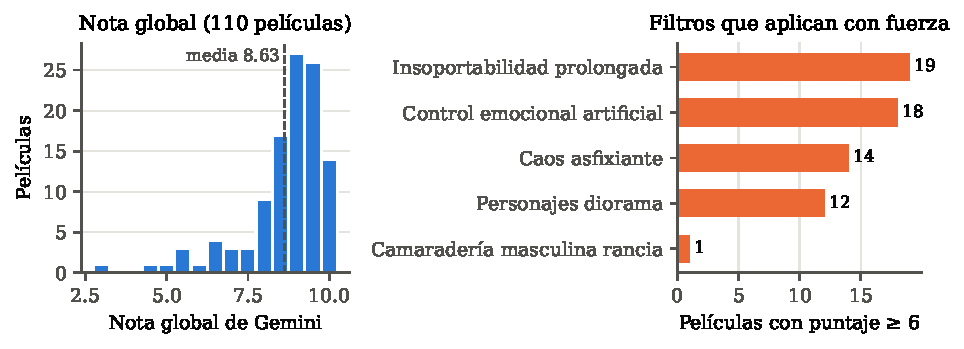
\includegraphics[width=\linewidth]{distribucion_verdad_base}
  \caption{La Verdad Base es una lista de películas preferidas: la nota media es 8.63 y 93 de 110 tienen 8 o más
  (izquierda). Los filtros casi nunca aplican con fuerza; \emph{Camaradería Masculina Rancia} tiene una sola película
  con puntaje $\geq 6$ (derecha).}
  \label{fig:distribucion}
\end{figure}

%=====================================================================
\section{El pipeline}
%=====================================================================

La figura~\ref{fig:pipeline} resume el flujo y la opción del menú (\texttt{python src/main.py}) que ejecuta cada paso.
Las secciones siguientes explican cada paso: qué hace, la estrategia elegida, la variante básica o alternativa
descartada y la evidencia para decidir. Todas las comparaciones se hicieron con validación cruzada repetida
(sección~\ref{sec:evaluacion}).

\begin{figure}[H]
\centering
\hyphenpenalty=10000 \exhyphenpenalty=10000 % sin cortes de palabra en las cajas
\begin{tikzpicture}[
    font=\small,
    caja/.style={draw=tinta2, rounded corners=3pt, fill=white, align=center, minimum height=9mm, inner sep=4pt, text width=#1},
    caja/.default=3.1cm,
    datos/.style={caja=2.9cm, fill=fondo},
    flecha/.style={-{Stealth[length=2.2mm]}, thick, tinta2},
    etiqueta/.style={font=\scriptsize\sffamily\bfseries, text=azul}]
  % Columna de reseñas
  \node[datos] (db) {Reseñas Letterboxd\\\scriptsize\archivo{reviews.db}};
  \node[caja, below=6mm of db] (filtro) {Filtrado\\\scriptsize$\geq$100 caracteres, 100 con más likes};
  \node[caja, below=6mm of filtro] (emb) {Chunks de 128 tokens\\ y embeddings e5};
  \node[caja, below=6mm of emb] (pool) {Resumen por película\\\scriptsize promedio de los chunks};
  % Columna del perfil
  \node[datos, right=1.6cm of db] (perfil) {Perfil JSON\\\scriptsize criterios, excepciones, frases};
  \node[caja, below=6mm of perfil] (embp) {Embeddings del perfil\\\scriptsize descripción y frases};
  \node[caja, below=6mm of embp] (rasgos) {Rasgos de frases\\\scriptsize cuántos chunks se parecen};
  % Columna de la verdad base
  \node[datos, right=1.6cm of perfil] (gemini) {Gemini\\\scriptsize instrucciones del perfil};
  \node[caja, below=6mm of gemini] (gt) {Verdad Base\\\scriptsize puntajes por criterio y nota};
  % Modelo
  \node[caja=4.2cm, below=1.4cm of rasgos] (e1) {\textbf{Etapa 1}: Ridge por criterio\\\scriptsize reseñas $\rightarrow$ puntaje de cada afinidad, filtro y excepción};
  \node[caja=4.2cm, below=6mm of e1] (e2) {\textbf{Etapa 2}: regla global\\\scriptsize puntajes $\rightarrow$ nota 0--10};
  \node[caja=3.2cm, below=6mm of e2, fill=azul!10] (rank) {\textbf{Ranking} de candidatas};
  \node[caja=2.8cm, right=1.2cm of rank] (eval) {Evaluación\\\scriptsize 5 particiones $\times$ 10 repeticiones};
  % Flechas
  \draw[flecha] (db) -- (filtro); \draw[flecha] (filtro) -- (emb); \draw[flecha] (emb) -- (pool);
  \draw[flecha] (perfil) -- (embp); \draw[flecha] (embp) -- (rasgos);
  \draw[flecha] (gemini) -- (gt); \draw[flecha] (perfil.east) -- (gemini.west);
  \draw[flecha] (emb.east) -- (rasgos.west);
  \draw[flecha] (pool.south) |- (e1.west);
  \draw[flecha] (rasgos) -- (e1);
  \draw[flecha] (gt.south) |- (e1.east);
  \draw[flecha] (gt.south) |- (e2.east);
  \draw[flecha] (e1) -- (e2); \draw[flecha] (e2) -- (rank);
  \draw[flecha, dashed] (rank.east) -- (eval.west);
  % Opciones del menú
  \node[etiqueta, left=1mm of filtro] {2};
  \node[etiqueta, left=1mm of emb] {4};
  \node[etiqueta, left=1mm of perfil] {1};
  \node[etiqueta, left=1mm of embp] {3};
  \node[etiqueta, right=1mm of gt] {5, 6};
  \node[etiqueta, anchor=south east] at (e1.north west) {7};
  \node[etiqueta, left=1mm of rank] {8};
  \node[etiqueta, right=1mm of eval] {9};
\end{tikzpicture}
\caption{Pipeline. Los números azules son las opciones del menú; la \menu{9} ejecuta de la 2 a la 8 sin preguntas y
agrega las comparaciones y el análisis.}
\label{fig:pipeline}
\end{figure}

\subsection{Filtrado de reseñas (\menu{2}, \texttt{src/db/filtered/filter.py})}\label{sec:filtrado}

Lee la base SQLite con una consulta con funciones de ventana: por cada película toma las reseñas con más \emph{likes},
descartando las de menos de 100 caracteres (suelen ser chistes de una línea que no describen la película), y solo
películas con al menos 20 reseñas. Limpia caracteres especiales y deja \archivo{film_id} (el \emph{slug} de
Letterboxd), título, director, idioma, \emph{likes} y texto. Si el resultado es idéntico al último filtrado no crea otro
archivo, para no duplicar embeddings después.

\begin{decision}{}
Elegida & hasta \textbf{100 reseñas por película}, ordenadas por \emph{likes} (\archivo{MAX_RESENIAS_POR_PELICULA}). \\
Descartadas & 200 reseñas: ordena igual o peor y duplica el tiempo de generar embeddings (con MiniLM, 100 ordenó mejor
que 200 en las 10 repeticiones, $\Delta\rho=+0.021$). 50 reseñas: peor con los tres modelos (fig.~\ref{fig:pooling}). \\
\end{decision}

\subsection{Chunks y embeddings de reseñas (\menu{4}, \texttt{src/procesing\_reviews.py})}

Cada reseña se divide con \archivo{semchunk} en fragmentos de hasta 128 tokens y cada fragmento se convierte en un
vector (\emph{embedding}) con un modelo multilingüe de \archivo{sentence-transformers}. Los vectores se guardan en
ChromaDB (colección \archivo{resenias}); cada modelo en su propia carpeta (\archivo{src/db/embeddings/chroma_<modelo>/})
porque sus dimensiones no se pueden mezclar. El identificador de cada chunk incluye película, lote, reseña y número de
chunk, así que reprocesar un lote no duplica.

\begin{decision}{}
Elegida & \textbf{\texttt{intfloat/multilingual-e5-base}} (768 dimensiones), con el prefijo \texttt{"query: "} que exige
la familia e5. Por defecto desde la versión 1.3. \\
Básica (descartada) & \texttt{paraphrase-multilingual-MiniLM-L12-v2} (384 dimensiones), la de las versiones anteriores:
$\rho=0.605$ contra $0.674$ con e5 (tabla~\ref{tab:modelos}). Sigue disponible con la variable \archivo{MODELO_EMBEDDINGS}. \\
Alternativa & \texttt{paraphrase-multilingual-mpnet-base-v2}: mejora las afinidades pero no los filtros ($\rho=0.651$). \\
Costo & e5 y mpnet tardan unas 3 veces más por chunk: 1\,h\,40\,min en GitHub Actions para 55\,769 chunks, sin GPU. \\
\end{decision}

\subsection{Embeddings del perfil (\menu{3}, \texttt{src/procesing\_profiles.py})}

Cada afinidad y cada filtro se vectoriza con el mismo modelo, junto a un documento por excepción y uno por cada frase
de reseña (colección \archivo{perfiles}).

\begin{decision}{}
Elegida & vectorizar solo \textbf{nombre y descripción} de cada criterio. \\
Descartada & el texto completo del criterio (con sus afinidades corrompidas y su excepción): acercaba el vector del filtro a
los conceptos que se oponen a él. La similitud entre \emph{Insoportabilidad} y \emph{Ternura} bajó de 0.68 a 0.50 al
quitar ese texto. \\
\end{decision}

\subsection{Resumen de cada película (\emph{pooling}, \texttt{src/pooling.py})}

Una película tiene cientos de chunks; la etapa 1 necesita un solo vector por película.

\begin{decision}{}
Elegida & \textbf{promedio} de los embeddings de todos sus chunks (\archivo{POOLING_RESENIAS=media}). \\
Descartadas & percentil 50, 75, 90 o 95 de cada dimensión del embedding, y promedio más percentiles de la similitud de
los chunks con cada término del perfil. Con e5 ninguna ordena mejor que el promedio en 10 repeticiones (la mejor,
$\Delta\rho=+0.001$; el percentil 75, $-0.021$, peor en las 10). Con una sola partición el percentil 90 parecía ganar
($0.584$ contra $0.606$ de MAE), pero era ruido (fig.~\ref{fig:pooling}). Se pueden elegir con \archivo{POOLING_RESENIAS=pXX}. \\
\end{decision}

\subsection{Rasgos de frases de reseña (\texttt{src/pooling.py})}\label{sec:frases}

La descripción de un filtro está escrita como la escribiría un crítico (``control emocional artificial''); las reseñas
dicen ``Oscar bait''. Un experimento previo (\archivo{src/experimentos/sondas_filtros.py}) midió, para cada texto, qué
fracción de los chunks de cada película se parece mucho a él y la correlacionó con el puntaje de Gemini del filtro
(tabla~\ref{tab:sondas}): las frases con el vocabulario de las reseñas detectan mejor cuatro de los cinco filtros.

Para cada criterio con \archivo{frases_resenia}, y para cada texto $t$ (su descripción y cada frase), se calcula:
\begin{itemize}
  \item la \textbf{fracción de chunks} de la película con similitud coseno con $t$ mayor que el percentil 95 de esa
  similitud en una muestra de 20\,000 chunks de todas las películas (el umbral no usa notas), y
  \item el \textbf{percentil 90} de la similitud de los chunks de la película con $t$.
\end{itemize}
Con 3--4 frases por filtro son 8--10 rasgos. El umbral de cada texto se guarda con el modelo para medir igual a las
películas que se recomiendan después.

\begin{decision}{}
Elegida & \textbf{ponderar}: los rasgos se agregan al embedding y, tras estandarizar, se multiplican por
$\sqrt{768/k}$ ($k$ = cantidad de rasgos), para que pesen en conjunto lo mismo que las 768 dimensiones del embedding.
Con e5 mejora el orden en las 10 repeticiones ($\Delta\rho=+0.008$) y baja el MAE. \\
Descartadas & concatenarlos sin ponderar (Ridge los diluye: $+0.002$); usar solo las frases, sin el embedding ($+0.011$
en $\rho$ pero sube el MAE y con mpnet no se repite); y los controles con solo la descripción ($+0.000$ y $+0.005$), que
muestran que la ganancia viene de las frases y no solo de medir ``cuántas reseñas hablan de''. \\
\end{decision}

\subsection{Modelo de reglas en dos etapas (\menu{7})}\label{sec:modelo}

Implementado en \archivo{src/modelo_reglas.py} y entrenado por \archivo{src/scoring.py}.

\paragraph{Etapa 1: de las reseñas a los puntajes.} Para cada criterio $c$ (afinidad, filtro o excepción) una regresión
Ridge, con estandarización y la regularización elegida por validación cruzada interna
($\alpha\in[10^{-1},10^4]$), predice el puntaje de Gemini a partir del embedding promedio de la película y, si el
criterio tiene frases, de sus rasgos. Las predicciones se recortan a $[0,10]$ (a $[0,1]$ para las excepciones). Son
11\,579 coeficientes regularizados en total (768 + rasgos por criterio).

\paragraph{Etapa 2: de los puntajes a la nota.} La regla global del perfil se traduce a una fórmula con parámetros que
se aprenden de la Verdad Base:
\begin{equation}
  \text{nota} = b + \sum_{j\in\text{afinidades}} w_j\,A_j \;-\; \sum_{k\in\text{filtros}} d_k\,
  \sigma\!\big(1.5\,(F_k-u_k)\big)\,(1-E_k),
  \label{eq:regla}
\end{equation}
donde $A_j$, $F_k$ y $E_k$ son los puntajes de afinidades, filtros y excepciones, $w_j\in[0,2]$ el peso de cada
afinidad, $u_k$ el umbral desde el que el filtro $k$ ``se activa'', $d_k$ cuánto resta como máximo, y $\sigma$ la
sigmoide, que hace suave el umbral para poder optimizarlo. La excepción ($E_k=1$) anula el descuento. Se ajusta con
L-BFGS-B minimizando el error cuadrático, con tres inicios y una penalización L2 pequeña ($10^{-3}$) sobre los
descuentos. Tiene $1+n_A+2n_F$ parámetros: 16 para este perfil, y la misma forma sirve para cualquier perfil. La etapa 2
se entrena con las 110 películas de la Verdad Base, porque no necesita reseñas.

La regla aprendida con e5 es:
\begin{itemize}
\item Nota base = 4.19 + 0.08·Resistencia Femenina + 0.12·Contemplación Inmersiva + 0.16·Ternura y Empatía Radical + 0.09·Humanismo Social + 0.19·Vanguardia y Simbolismo
\item Si Insoportabilidad Prolongada supera 5.4 y su excepción no aplica: resta hasta 1.66 puntos.
\item Si Control Emocional Artificial supera 8.8 y su excepción no aplica: resta hasta 2.98 puntos.
\item Si Personajes Diorama supera 4.0 y su excepción no aplica: resta hasta 0.45 puntos.
\item Si Caos Asfixiante supera 0.9 y su excepción no aplica: resta hasta 0.25 puntos.
\end{itemize}


\begin{decision}{}
Elegida & \textbf{modelo de reglas} de dos etapas con la regla simple \eqref{eq:regla}. \\
Básica (descartada) & la \textbf{regresión lineal} de las versiones anteriores: similitud coseno entre el embedding de la
película y el de cada término del perfil, más un producto por relación (afinidad $\times$ filtro, filtro $\times$
excepción), 21 variables. Ordena peor ($\rho=0.546$ contra $0.674$ con e5) y con MiniLM su error era mayor que
predecir el promedio (MAE $0.828$ contra $0.812$). La \menu{9} la sigue calculando como comparación. \\
Alternativas de etapa 2 & regla con \emph{pisos} (una afinidad alta asegura una nota mínima) y \emph{corrupción} (el
filtro reduce las afinidades que corrompe): MAE $0.293$ contra $0.294$ con casi el doble de parámetros (31); quedan como
opciones desactivadas. También se probaron regresión lineal ($0.333$), GAM, \emph{gradient boosting} con y sin
restricciones monótonas y \emph{random forest} (peores con 110 películas) y la regla corregida con \emph{boosting}
($0.280$, apenas mejor y mucho menos legible). \\
\end{decision}

\subsection{Recomendación (\menu{8}, \texttt{src/recommend.py})}

Carga el modelo guardado por la \menu{7} (\archivo{src/loss/modelo_reglas_<modelo>.joblib}, con el pooling, las
frases y sus umbrales) y ordena todas las películas con reseñas por la nota predicha. Las que ya tienen nota de Gemini
aparecen para comparar.

\subsection{Evaluación (\menu{9}, \texttt{src/analisis.py}, \texttt{src/metricas.py})}\label{sec:evaluacion}

\begin{itemize}
  \item \textbf{Validación cruzada}: cada película se predice con un modelo que no la vio. 5 particiones, repetidas con
  10 semillas distintas; se informa el promedio y la desviación. Con unas 100 películas, el $\rho$ de una sola partición
  varía $\pm 0.05$, tanto como las diferencias que se quieren medir.
  \item \textbf{Comparaciones pareadas}: cada variante se compara contra una referencia \emph{en las mismas
  particiones} ($\Delta\rho$), que varía mucho menos, y se cuenta en cuántas de las 10 repeticiones la supera.
  \item \textbf{Métricas}: $\rho$ de Spearman (principal: el orden completo); NDCG@10 (si las 10 primeras según el
  modelo son las mejores según Gemini, en ese orden, con ganancia $y-\min y$); precisión@10 (fracción de las 10
  primeras que están entre las 10 mejores, contando empates en el corte), y MAE de la nota. La línea base (predecir el
  promedio) se informa con los valores esperados de un orden al azar.
\end{itemize}

\begin{decision}{}
Elegida & $\rho$ de Spearman como métrica principal, promedio de 10 repeticiones. \\
Descartada & MAE como métrica principal y una sola partición: favorecía variantes que no ordenan mejor (las frases de
reseña casi no cambian el MAE pero sí el orden) y hacía que variantes iguales parecieran distintas. \\
\end{decision}

%=====================================================================
\section{Ejemplo guiado: \emph{Manhattan} (Woody Allen, 1979)}\label{sec:ejemplo}
%=====================================================================

\emph{Manhattan} es una de las pocas películas de la lista con nota baja (Gemini: \EjNotaGemini) y la razón es un
filtro: la película obliga a convivir con un protagonista cuya relación con una adolescente de 17 años y cuyo aire de
superioridad intelectual encajan en \emph{Insoportabilidad Prolongada} (Gemini: \EjInsGemini{} de 10, sin excepción).
Además Gemini le da puntajes bajos en tres afinidades. Es un caso difícil y por eso instructivo: muestra cada paso y
también dónde falla el modelo. Para que el ejemplo sea honesto, el modelo de esta sección se entrenó \textbf{con todas
las demás películas y sin Manhattan}, como si fuera una candidata nueva.

\paragraph{Paso 1: reseñas.} El filtrado toma sus \EjResenias{} reseñas con más \emph{likes} y al menos 100 caracteres,
en inglés, portugués, persa, árabe y otros idiomas. Entre ellas hay críticas al personaje, que mencionan su edad y lo
tratan de \emph{pretentious} y \emph{creep}, pero son una minoría frente a las que elogian la fotografía en blanco y negro
y la música de Gershwin.

\paragraph{Paso 2: chunks y embeddings.} Las reseñas se dividen en \EjChunks{} chunks de hasta 128 tokens y cada uno se
convierte en un vector de 768 dimensiones con e5. El promedio de esos vectores es la representación de la película. En
el promedio, las críticas de la minoría se diluyen: para eso están los rasgos de frases.

\paragraph{Paso 3: rasgos de frases.} Para \emph{Insoportabilidad Prolongada}, la tabla~\ref{tab:ejemplo_frases} muestra
qué fracción de los chunks de Manhattan supera el umbral de similitud con cada texto. Con la frase \emph{``I couldn't
stand the protagonist, he is a pretentious narcissist and a creep''}, el \EjFraseManhattan\,\% de sus chunks la supera,
contra \EjFraseMediana\,\% en la película mediana: Manhattan está en el percentil \EjFrasePercentil{} de las 101 películas.
Con la descripción del perfil, escrita en otro registro, queda en el percentil \EjDescPercentil. Las frases sí encuentran
el problema.

\begin{table}[H]
  \centering\small
  \begin{tabular}{>{\raggedright\arraybackslash}p{7.2cm}ccc}
\toprule
Texto & Manhattan & Mediana & Percentil \\
\midrule
\emph{descripción} & 2.1\,\% & 3.8\,\% & 26 \\
\emph{the main character is insufferable, arrogant and smug} & 7.3\,\% & 4.6\,\% & 85 \\
\emph{I couldn't stand the protagonist, he is a pretentious narcissist and a creep} & 11.5\,\% & 4.2\,\% & 95 \\
\emph{an unlikable, annoying character you have to spend the whole movie with} & 5.6\,\% & 4.7\,\% & 65 \\
\emph{un protagonista insoportable, arrogante y pedante} & 6.3\,\% & 4.1\,\% & 67 \\
\bottomrule
\end{tabular}

  \caption{Rasgos de frases de \emph{Insoportabilidad Prolongada} para Manhattan: fracción de sus chunks sobre el
  umbral de cada texto, la misma fracción en la película mediana y el percentil de Manhattan entre las 101 películas.}
  \label{tab:ejemplo_frases}
\end{table}

\paragraph{Pasos 4 y 5: etapa 1 y regla global.} La etapa 1 predice los 14 puntajes desde el embedding y los rasgos, y la
regla \eqref{eq:regla} los combina (tabla~\ref{tab:ejemplo}). La nota base es $b+\sum_j w_jA_j=\EjBase$ y los filtros
restan \EjDescuento{} en total: la nota predicha queda en \textbf{\EjNotaModelo}, lejos del \EjNotaGemini{} de Gemini.

\begin{table}[H]
  \centering\footnotesize
  \begin{tabular}{lcccr}
\toprule
Criterio & Gemini & Etapa 1 (predicho) & Parámetros de la regla & Aporte \\
\midrule
Sesgo & & & & 3.74 \\
Resistencia Femenina & 2.0 & 7.0 & $w$ = 0.10 & +0.69 \\
Contemplación Inmersiva & 6.0 & 7.0 & $w$ = 0.11 & +0.74 \\
Ternura y Empatía Radical & 2.0 & 7.2 & $w$ = 0.15 & +1.09 \\
Humanismo Social & 3.0 & 6.2 & $w$ = 0.13 & +0.79 \\
Vanguardia y Simbolismo & 6.0 & 6.3 & $w$ = 0.20 & +1.26 \\
\midrule
Camaradería Masculina Rancia & 9.0 (exc. 1) & 0.3 (exc. 0.11) & $u$ = 4.9, $d$ = 0.05, act. 0.00 & 0.00 \\
Insoportabilidad Prolongada & 8.0 (exc. 0) & 3.0 (exc. 0.36) & $u$ = 5.6, $d$ = 1.68, act. 0.01 & $-$0.02 \\
Control Emocional Artificial & 3.0 (exc. 0) & 2.9 (exc. 0.00) & $u$ = 8.8, $d$ = 2.16, act. 0.00 & 0.00 \\
Personajes Diorama & 4.0 (exc. 0) & 3.3 (exc. 0.01) & $u$ = 7.1, $d$ = 0.65, act. 0.00 & 0.00 \\
Caos Asfixiante & 0.0 (exc. 0) & 0.0 (exc. 0.00) & $u$ = 2.2, $d$ = 0.24, act. 0.04 & $-$0.01 \\
\midrule
\multicolumn{4}{l}{\textbf{Nota predicha} (Gemini: 5.0)} & \textbf{8.28} \\
\bottomrule
\end{tabular}

  \caption{Cálculo de la nota de Manhattan con el modelo entrenado sin ella. Para los filtros, ``act.'' es
  $\sigma(1.5(F_k-u_k))(1-E_k)$, la fracción del descuento $d_k$ que se aplica; ``exc.'' es la excepción.}
  \label{tab:ejemplo}
\end{table}

\paragraph{Dónde falla.} La etapa 2 hace lo que dice la regla, pero recibe puntajes equivocados de la etapa 1:
\begin{itemize}
  \item \textbf{Afinidades}: la etapa 1 predice cerca de 7 para todas, el valor típico de la lista, mientras Gemini da 2
  o 3 en tres de ellas. Con 101 películas casi todas bien evaluadas, Ridge aprende a quedarse cerca del promedio.
  \item \textbf{El filtro}: aunque el rasgo de la frase está en el percentil \EjFrasePercentil, la etapa 1 predice
  \EjInsPredicho{} para \emph{Insoportabilidad}, bajo su umbral de \EjInsUmbral, y el descuento no se activa. Hay 19
  películas con ese filtro alto: pocas para que Ridge le dé tanto peso al rasgo.
  \item \textbf{Camaradería Masculina Rancia}: Gemini le da 9, pero con su excepción aplicada; Manhattan es la
  \emph{única} película de la lista con ese filtro alto, así que al sacarla del entrenamiento no queda ningún ejemplo.
\end{itemize}

\paragraph{En el ranking.} En la validación cruzada de 10 repeticiones, Manhattan queda en el puesto
\PuestoManhattan{} de \NPeliculasCV{} (nota predicha \NotaCVManhattan; en Gemini es la \PuestoGeminiManhattan). El caso
contrario es \emph{Marty Supreme} (Gemini \NotaGeminiMarty, puesto \PuestoGeminiMarty): el modelo la deja última
(\PuestoMarty{} de \NPeliculasCV, nota \NotaCVMarty). \emph{Amélie} (\NotaGeminiAmelie, la peor nota con reseñas) queda en
el puesto \PuestoAmelie: sus reseñas describen lo dulce y excéntrico como virtud, mientras el perfil lo considera
\emph{Control Emocional Artificial}. Los errores grandes se concentran en películas cuyo defecto, según el perfil, las
reseñas no describen como defecto, o describen en pocas reseñas. Más películas con notas bajas en la Verdad Base
atacarían ambos problemas (sección~\ref{sec:pasos}).

%=====================================================================
\section{Cómo ejecutarlo}
%=====================================================================

\subsection{Instalación y datos}
\begin{Verbatim}[fontsize=\small,frame=single,framesep=2mm]
pip install -r requirements.txt
# perfil de ejemplo:
cp src/db/profiles/perfiles.ejemplo.json src/db/profiles/perfiles.json
python src/main.py
\end{Verbatim}

\begin{enumerate}
  \item Descargar del \emph{release} en borrador \archivo{datos-resenas} el archivo \archivo{reviews.zip} y
  descomprimirlo en \archivo{src/db/raw/} (queda \archivo{reviews.db}).
  \item \textbf{Embeddings}: generarlos en CPU con e5 (opciones 2 a 4) tarda varias horas. El mismo \emph{release} tiene
  la base ya generada, \archivo{embeddings-multilingual-e5-base-100-<huella>.zip}: descomprimirla en la raíz del
  repositorio. Crea \archivo{src/db/embeddings/chroma_multilingual-e5-base/} y el CSV filtrado correspondiente; las
  opciones 2 y 4 reconocen que ya están procesados.
  \item Ejecutar la \menu{9} (todo el pipeline y el análisis), o las opciones 3, 5, 7 y 8 por separado.
\end{enumerate}

\subsection{Menú principal}
\noindent\begin{tabularx}{\linewidth}{@{}l>{\raggedright\arraybackslash}X@{}}
\toprule
Opción & Qué hace \\ \midrule
1 & Crear o editar perfiles: criterios, excepciones, encabezados, regla global y frases de reseña. \\
2 & Filtrar las reseñas crudas (\archivo{src/db/raw/*.db} o \archivo{*.csv}). \\
3 & Embeddings del perfil (descripciones, excepciones y frases). \\
4 & Embeddings de los lotes de reseñas pendientes. \\
5 & Cargar la Verdad Base desde \archivo{dataset_maestro.csv} y las evaluaciones adicionales. \\
6 & Listar películas con reseñas sin nota y generar la plantilla y las instrucciones para Gemini. \\
7 & Entrenar el modelo de reglas; informa $\rho$, NDCG@10, precisión@10 y MAE en validación cruzada y las reglas aprendidas. \\
8 & Ranking de recomendaciones con el modelo guardado. \\
9 & Ejecutar de la 2 a la 8 sin preguntas y guardar el análisis en \archivo{analisis/<fecha>_<modelo>/}. \\
10 & Salir. \\ \bottomrule
\end{tabularx}

\subsection{Variables de entorno}
\noindent\begin{tabularx}{\linewidth}{@{}l>{\raggedright\arraybackslash}X@{}}
\toprule
Variable & Uso \\ \midrule
\archivo{MODELO_EMBEDDINGS} & Modelo de embeddings (por defecto \texttt{intfloat/multilingual-e5-base}). \\
\archivo{MAX_RESENIAS_POR_PELICULA} & Reseñas por película (por defecto 100). \\
\archivo{POOLING_RESENIAS} & \texttt{media} (por defecto) o \texttt{pXX}. El modelo guardado recuerda cuál usó. \\ \bottomrule
\end{tabularx}

\subsection{GitHub Actions}
\begin{itemize}
  \item \archivo{analisis.yml}: ejecuta la \menu{9} con MiniLM, mpnet y e5 en paralelo, reutiliza los embeddings del
  caché y publica los resultados en la rama \archivo{resultados-analisis} (solo números, nunca texto de reseñas). El job
  de e5 publica su base de embeddings en el \emph{release} en borrador. Corre al cambiar el workflow, el perfil de
  ejemplo, \archivo{analisis.py}, \archivo{modelo_reglas.py} o \archivo{pooling.py}.
  \item \archivo{sondas.yml}: el experimento de frases sonda de la sección~\ref{sec:frases}.
  \item \archivo{tests.yml}: en cada \emph{push}, 30 pruebas unitarias con datos sintéticos
  (\texttt{python -m pytest tests}) y la revisión estática del código con \archivo{pyflakes}.
\end{itemize}

\subsection{Archivos del análisis}
\archivo{resumen.md} (todas las tablas), \archivo{peliculas.csv} (por película: similitudes, puntajes predichos, notas y
errores), \archivo{ranking.csv}, \archivo{reglas.json}, \archivo{pooling.csv}, \archivo{frases_resenia.csv},
\archivo{pesos.csv} y \archivo{similitud_perfil.csv}. Este informe se regenera con
\texttt{python docs/informe/figuras.py}, \texttt{python docs/informe/tablas.py} y \texttt{latexmk -pdf informe.tex}
desde \archivo{docs/informe/}.

%=====================================================================
\section{Resultados}
%=====================================================================

Las tablas~\ref{tab:modelos} a~\ref{tab:candidatas} y las figuras~\ref{fig:pooling} y~\ref{fig:frases} vienen de la
corrida del workflow de análisis del 26 de septiembre (commit \texttt{9669c1c}), publicada en la rama
\archivo{resultados-analisis}. La curva de aprendizaje, la dispersión y el ejemplo guiado se calcularon con el mismo código
sobre la base de embeddings de e5 publicada en el \emph{release}. Los datos agregados de cada tabla y figura están en
\archivo{docs/informe/datos/}.

\subsection{Modelo final y comparación de modelos de embeddings}

\begin{table}[H]
  \centering\footnotesize
  \begin{tabular}{llcccc}
\toprule
Embeddings & Modelo & $\rho$ Spearman & NDCG@10 & Precisión@10 & MAE \\
\midrule
\multirow{3}{*}{MiniLM} & \textbf{Reglas + frases (op.~7 y 8)} & \textbf{0.605} $\pm$ 0.024 & 0.929 & 0.280 & 0.632 \\
 & Regresión lineal anterior & 0.464 & 0.909 & 0.200 & 0.828 \\
 & Regresión lineal con Ridge & 0.400 & 0.886 & 0.300 & 0.809 \\ \midrule
\multirow{3}{*}{mpnet-base} & \textbf{Reglas + frases (op.~7 y 8)} & \textbf{0.651} $\pm$ 0.024 & 0.934 & 0.260 & 0.601 \\
 & Regresión lineal anterior & 0.598 & 0.906 & 0.200 & 0.891 \\
 & Regresión lineal con Ridge & 0.605 & 0.906 & 0.300 & 0.745 \\ \midrule
\multirow{3}{*}{e5-base} & \textbf{Reglas + frases (op.~7 y 8)} & \textbf{0.674} $\pm$ 0.026 & 0.938 & 0.280 & 0.580 \\
 & Regresión lineal anterior & 0.546 & 0.897 & 0.300 & 0.735 \\
 & Regresión lineal con Ridge & 0.597 & 0.944 & 0.500 & 0.659 \\ \midrule
\multicolumn{2}{l}{Orden al azar / predecir el promedio} & 0 & 0.780 & 0.129 & 0.812 \\
\bottomrule
\end{tabular}

  \caption{Validación cruzada (101 películas). El modelo de reglas es el promedio de 10 repeticiones $\pm$ su
  desviación; las regresiones lineales, una partición. En negrita, el modelo que usan las opciones 7 y 8.}
  \label{tab:modelos}
\end{table}

\begin{figure}[H]
  \centering
  \begin{minipage}[t]{0.56\linewidth}\vspace{0pt}
    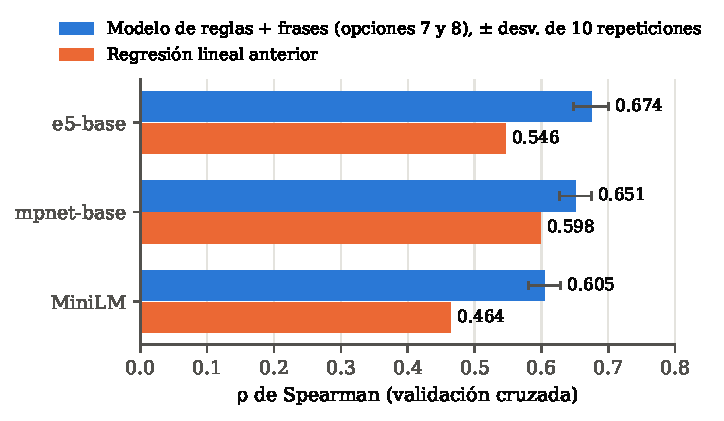
\includegraphics[width=\linewidth]{modelos}
  \end{minipage}\hfill
  \begin{minipage}[t]{0.42\linewidth}\vspace{0pt}
    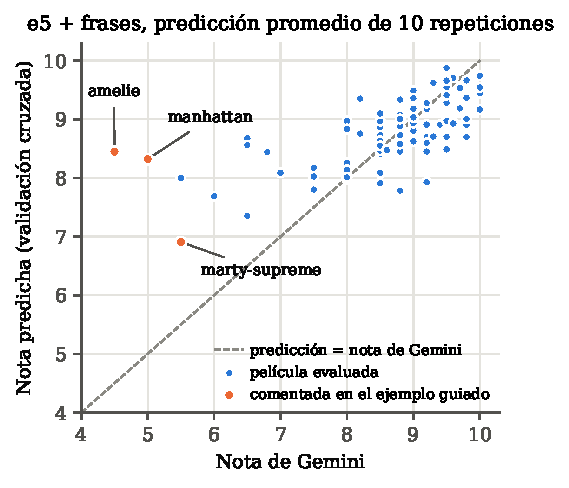
\includegraphics[width=\linewidth]{dispersion}
  \end{minipage}
  \caption{Izquierda: $\rho$ de Spearman por modelo de embeddings (datos de la tabla~\ref{tab:modelos}). Derecha: nota
  de Gemini contra la nota predicha en validación cruzada con e5; en naranja, películas comentadas en el texto. El
  modelo comprime las notas hacia el promedio: sube las peores y baja las mejores, pero conserva buena parte del orden.}
  \label{fig:modelos}
\end{figure}

\subsection{Dónde se pierde precisión: la etapa 1}

Con los puntajes reales de Gemini, la etapa 2 explica el 88\,\% de la varianza de la nota global
(tabla~\ref{tab:etapa2}). Con los puntajes que predice la etapa 1 desde las reseñas, el modelo completo explica el
39\,\%. El cuello de botella es predecir los criterios desde las reseñas, sobre todo los filtros
(fig.~\ref{fig:etapa1}).

\begin{table}[H]
  \centering\small
  \begin{tabular}{lccc}
\toprule
Entrada de la etapa 2 & $\rho$ Spearman & $R^2$ & MAE \\
\midrule
\multicolumn{4}{l}{\emph{Puntajes reales de Gemini (110 películas)}} \\
Regla con condiciones (16 parámetros) & 0.904 & 0.882 & 0.317 \\
Regresión lineal sobre los puntajes & 0.898 & 0.881 & 0.325 \\
Predecir el promedio & 0.000 & -0.013 & 0.911 \\
\midrule
Modelo completo (etapa 1 desde reseñas + regla), e5 & 0.674 & 0.394 & 0.580 \\
\bottomrule
\end{tabular}

  \caption{Etapa 2 por separado (validación cruzada sobre los puntajes de Gemini) y modelo completo.}
  \label{tab:etapa2}
\end{table}

\begin{figure}[H]
  \centering
  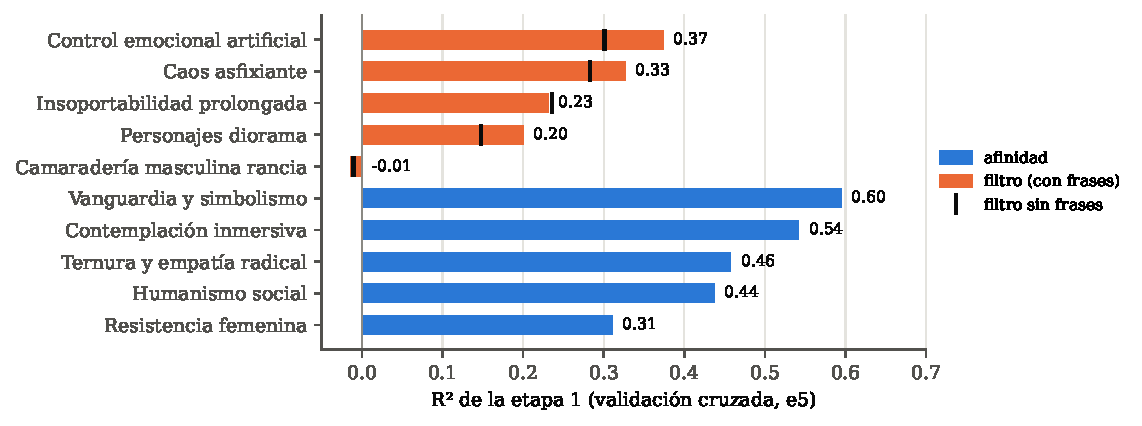
\includegraphics[width=0.95\linewidth]{etapa_1}
  \caption{$R^2$ de la etapa 1 por criterio (e5). Las afinidades se predicen mejor que los filtros; las frases de reseña
  mejoran los filtros (barra) respecto del modelo sin frases (marca negra). \emph{Camaradería Masculina Rancia} no se
  puede aprender: una sola película con puntaje alto.}
  \label{fig:etapa1}
\end{figure}

\subsection{Pooling y cantidad de reseñas}

\begin{figure}[H]
  \centering
  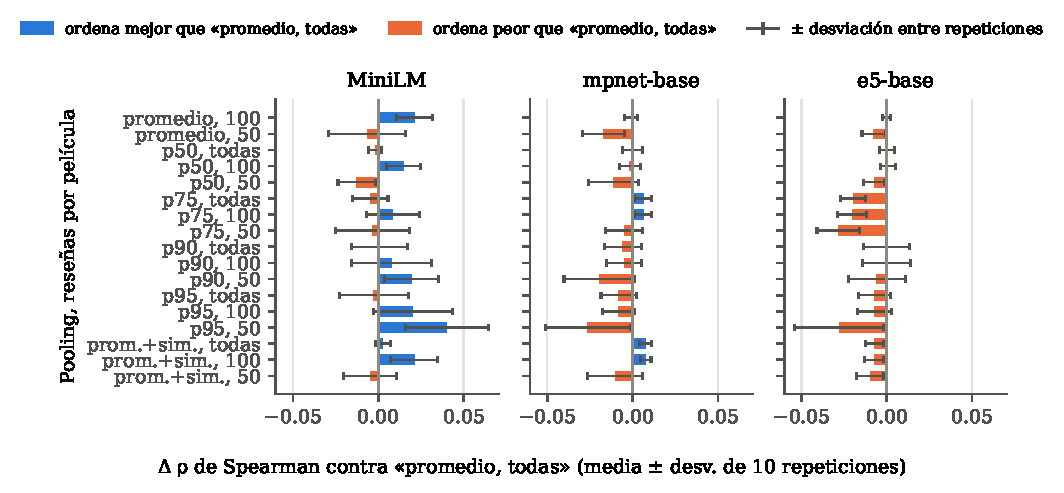
\includegraphics[width=\linewidth]{pooling}
  \caption{Diferencia de $\rho$ de cada forma de resumir las reseñas contra el promedio de todas (media $\pm$ desviación
  de 10 repeticiones pareadas). Con mpnet y e5 ``todas'' son 100 reseñas. Ninguna variante mejora de forma consistente
  con los tres modelos; con e5, el promedio es el mejor.}
  \label{fig:pooling}
\end{figure}

\begin{table}[H]
  \centering\scriptsize
  \begin{tabular}{lrcrcrc}
\toprule
Variante & \multicolumn{2}{c}{MiniLM} & \multicolumn{2}{c}{mpnet-base} & \multicolumn{2}{c}{e5-base} \\
\cmidrule(lr){2-3}\cmidrule(lr){4-5}\cmidrule(lr){6-7}
 & $\Delta\rho$ & mejora & $\Delta\rho$ & mejora & $\Delta\rho$ & mejora \\
\midrule
promedio, todas (elegida) & \multicolumn{2}{c}{$\rho$ = 0.596 (ref.)} & \multicolumn{2}{c}{$\rho$ = 0.644 (ref.)} & \multicolumn{2}{c}{$\rho$ = 0.667 (ref.)} \\
promedio, 100 & \textbf{+0.021} $\pm$ 0.011 & 10/10 & -0.001 $\pm$ 0.004 & 3/10 & -0.000 $\pm$ 0.002 & 4/10 \\
promedio, 50 & -0.006 $\pm$ 0.023 & 5/10 & -0.017 $\pm$ 0.012 & 1/10 & -0.008 $\pm$ 0.007 & 1/10 \\
percentil 50, todas & -0.002 $\pm$ 0.004 & 3/10 & -0.000 $\pm$ 0.006 & 5/10 & +0.000 $\pm$ 0.004 & 5/10 \\
percentil 50, 100 & \textbf{+0.015} $\pm$ 0.010 & 9/10 & -0.002 $\pm$ 0.006 & 4/10 & +0.000 $\pm$ 0.004 & 6/10 \\
percentil 50, 50 & -0.013 $\pm$ 0.011 & 1/10 & -0.011 $\pm$ 0.015 & 3/10 & -0.007 $\pm$ 0.006 & 1/10 \\
percentil 75, todas & -0.005 $\pm$ 0.010 & 4/10 & \textbf{+0.006} $\pm$ 0.005 & 9/10 & -0.020 $\pm$ 0.007 & 0/10 \\
percentil 75, 100 & +0.008 $\pm$ 0.016 & 6/10 & \textbf{+0.006} $\pm$ 0.005 & 9/10 & -0.020 $\pm$ 0.009 & 0/10 \\
percentil 75, 50 & -0.003 $\pm$ 0.022 & 5/10 & -0.005 $\pm$ 0.011 & 3/10 & -0.028 $\pm$ 0.013 & 0/10 \\
percentil 90, todas & +0.001 $\pm$ 0.016 & 5/10 & -0.006 $\pm$ 0.011 & 4/10 & -0.000 $\pm$ 0.013 & 5/10 \\
percentil 90, 100 & +0.008 $\pm$ 0.024 & 7/10 & -0.005 $\pm$ 0.010 & 5/10 & -0.000 $\pm$ 0.014 & 5/10 \\
percentil 90, 50 & \textbf{+0.019} $\pm$ 0.016 & 9/10 & -0.020 $\pm$ 0.021 & 2/10 & -0.006 $\pm$ 0.017 & 4/10 \\
percentil 95, todas & -0.003 $\pm$ 0.020 & 5/10 & -0.008 $\pm$ 0.010 & 3/10 & -0.007 $\pm$ 0.010 & 3/10 \\
percentil 95, 100 & +0.020 $\pm$ 0.023 & 8/10 & -0.008 $\pm$ 0.009 & 2/10 & -0.007 $\pm$ 0.010 & 3/10 \\
percentil 95, 50 & \textbf{+0.040} $\pm$ 0.024 & 9/10 & -0.026 $\pm$ 0.025 & 2/10 & -0.028 $\pm$ 0.026 & 2/10 \\
promedio + sim., todas & +0.003 $\pm$ 0.004 & 7/10 & \textbf{+0.008} $\pm$ 0.003 & 10/10 & -0.007 $\pm$ 0.005 & 0/10 \\
promedio + sim., 100 & \textbf{+0.021} $\pm$ 0.014 & 10/10 & \textbf{+0.008} $\pm$ 0.003 & 10/10 & -0.007 $\pm$ 0.006 & 1/10 \\
promedio + sim., 50 & -0.005 $\pm$ 0.016 & 3/10 & -0.010 $\pm$ 0.016 & 2/10 & -0.010 $\pm$ 0.008 & 1/10 \\
\bottomrule
\end{tabular}

  \caption{Datos de la figura~\ref{fig:pooling}: $\Delta\rho$ media $\pm$ desviación y repeticiones (de 10) en que la
  variante supera a la referencia. En negrita, mejoras en al menos 9 de 10.}
  \label{tab:pooling}
\end{table}

\subsection{Frases de reseña}

\begin{table}[H]
  \centering\footnotesize
  \begin{tabular}{lcccp{4.6cm}}
\toprule
Filtro & Descripción & Mejor frase & Léxico & Frase con mejor $\rho$ \\
\midrule
Camaradería Masculina Rancia & 0.01 & 0.08 & -0.03 & \emph{``humor machista y sexista, las mujeres son un chiste''} \\
Insoportabilidad Prolongada & 0.39 & 0.53 & 0.55 & \emph{``I couldn't stand the protagonist, he is a pretentious narcissist and a creep''} \\
Control Emocional Artificial & -0.04 & 0.40 & 0.16 & \emph{``Oscar bait designed to make you cry''} \\
Personajes Diorama & 0.03 & 0.28 & 0.17 & \emph{``style over substance, the characters feel like dolls in a dollhouse''} \\
Caos Asfixiante & 0.30 & 0.17 & 0.34 & \emph{``overstimulating, loud and relentless, too much happening at once''} \\
\bottomrule
\end{tabular}

  \caption{Experimento de frases sonda (MiniLM, 101 películas): $\rho$ de Spearman entre la fracción de chunks muy
  similares a cada texto y el puntaje de Gemini del filtro, y la correlación de un conteo de palabras clave (léxico).
  La descripción del perfil, escrita como la escribiría un crítico, detecta mal \emph{Control} y \emph{Diorama}.}
  \label{tab:sondas}
\end{table}

\begin{figure}[H]
  \centering
  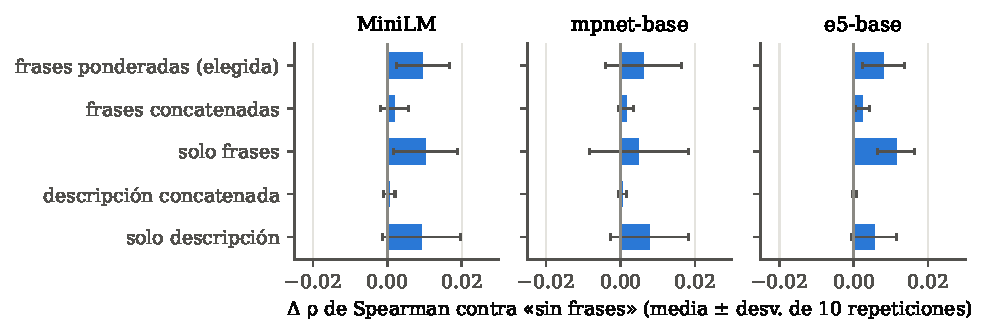
\includegraphics[width=\linewidth]{frases}
  \caption{Diferencia de $\rho$ de cada forma de usar las frases contra el modelo sin frases (10 repeticiones
  pareadas). Con e5, las frases ponderadas mejoran en las 10 repeticiones.}
  \label{fig:frases}
\end{figure}

\begin{table}[H]
  \centering\scriptsize
  \begin{tabular}{lrcrcrc}
\toprule
Variante & \multicolumn{2}{c}{MiniLM} & \multicolumn{2}{c}{mpnet-base} & \multicolumn{2}{c}{e5-base} \\
\cmidrule(lr){2-3}\cmidrule(lr){4-5}\cmidrule(lr){6-7}
 & $\Delta\rho$ & mejora & $\Delta\rho$ & mejora & $\Delta\rho$ & mejora \\
\midrule
sin frases (referencia) & \multicolumn{2}{c}{$\rho$ = 0.596 (ref.)} & \multicolumn{2}{c}{$\rho$ = 0.644 (ref.)} & \multicolumn{2}{c}{$\rho$ = 0.667 (ref.)} \\
frases ponderadas (elegida) & \textbf{+0.010} $\pm$ 0.007 & 9/10 & +0.006 $\pm$ 0.010 & 7/10 & \textbf{+0.008} $\pm$ 0.006 & 10/10 \\
frases concatenadas & +0.002 $\pm$ 0.004 & 7/10 & +0.001 $\pm$ 0.002 & 6/10 & \textbf{+0.002} $\pm$ 0.002 & 10/10 \\
solo frases & \textbf{+0.010} $\pm$ 0.009 & 10/10 & +0.005 $\pm$ 0.013 & 5/10 & \textbf{+0.011} $\pm$ 0.005 & 10/10 \\
descripción concat. (control) & +0.001 $\pm$ 0.001 & 8/10 & +0.001 $\pm$ 0.001 & 8/10 & +0.000 $\pm$ 0.000 & 8/10 \\
solo descripción (control) & +0.009 $\pm$ 0.011 & 8/10 & +0.008 $\pm$ 0.010 & 7/10 & +0.005 $\pm$ 0.006 & 7/10 \\
\bottomrule
\end{tabular}

  \caption{Datos de la figura~\ref{fig:frases}. En negrita, mejoras en al menos 9 de 10 repeticiones.}
  \label{tab:frases}
\end{table}

\subsection{¿Cuánto ayudaría tener más películas evaluadas?}

La curva de aprendizaje (fig.~\ref{fig:curva}) entrena con una fracción de las películas de cada partición y predice el
resto. $\rho$ sube de 0.45 con 20 películas a 0.60 con 40, 0.65 con 61 y 0.675 con 81: todavía sube, pero cada vez menos
($+0.026$ entre 61 y 81). Más películas parecidas a las actuales darían una mejora moderada; películas con notas bajas
y con los filtros presentes deberían rendir más, porque aportan justo la variedad que falta (sección~\ref{sec:pasos}).

\begin{figure}[H]
  \centering
  \begin{minipage}[c]{0.55\linewidth}
    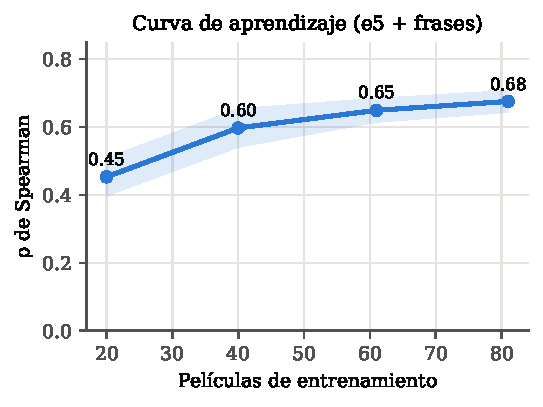
\includegraphics[width=\linewidth]{curva_aprendizaje}
  \end{minipage}\hfill
  \begin{minipage}[c]{0.4\linewidth}\centering\footnotesize
    \begin{tabular}{cc}
\toprule
Películas & $\rho$ Spearman \\
\midrule
20 & 0.453 $\pm$ 0.056 \\
40 & 0.597 $\pm$ 0.057 \\
61 & 0.649 $\pm$ 0.035 \\
81 & 0.675 $\pm$ 0.032 \\
\bottomrule
\end{tabular}

  \end{minipage}
  \caption{Curva de aprendizaje (e5 + frases, 5 particiones $\times$ 10 repeticiones): $\rho$ medio $\pm$ desviación
  según la cantidad de películas de entrenamiento.}
  \label{fig:curva}
\end{figure}

\subsection{Recomendaciones}

\begin{table}[H]
  \centering\small
  \begin{tabular}{rlcc}
\toprule
\# & Película & Nota del modelo & Nota lineal anterior \\
\midrule
1 & \texttt{taipei-suicide-story} & 9.75 & 10.30 \\
2 & \texttt{under-the-skin} & 9.52 & 9.42 \\
3 & \texttt{train-dreams} & 9.45 & 9.49 \\
4 & \texttt{2046} & 9.43 & 8.53 \\
5 & \texttt{the-passion-of-joan-of-arc} & 9.32 & 8.64 \\
6 & \texttt{the-seventh-seal} & 9.30 & 10.17 \\
7 & \texttt{sentimental-value} & 9.29 & 8.56 \\
8 & \texttt{happy-together} & 9.23 & 9.15 \\
9 & \texttt{chungking-express} & 9.18 & 8.50 \\
10 & \texttt{neon-genesis-evangelion} & 9.12 & 8.97 \\
\bottomrule
\end{tabular}

  \caption{Las 10 mejores candidatas (sin nota de Gemini) según el modelo de reglas con e5, y la nota que les daba la
  regresión lineal anterior.}
  \label{tab:candidatas}
\end{table}

%=====================================================================
\section{Observaciones}
%=====================================================================

\begin{enumerate}
  \item \textbf{La Verdad Base es una lista de películas preferidas.} Con media 8.63 y 93 de 110 películas con 8 o más,
  el modelo aprende sobre todo a distinguir ``muy buena'' de ``excelente''. Los filtros casi nunca aplican
  (fig.~\ref{fig:distribucion}), así que hay pocos ejemplos para aprender a detectarlos, y \emph{Camaradería Masculina
  Rancia} tiene uno solo. El rango estrecho también limita el $\rho$ alcanzable: con notas casi iguales, pequeñas
  diferencias cambian el orden.
  \item \textbf{La Verdad Base es la lectura de Gemini, no la nota de la persona.} El modelo aprende a imitar cómo
  Gemini interpreta el perfil. Falta medir cuánto se parece eso al gusto real y cuán consistente es Gemini consigo
  mismo: si al reevaluar las mismas películas su propio $\rho$ ronda 0.8, el 0.67 del modelo estaría cerca del techo.
  \item \textbf{El cuello de botella es la etapa 1} (tabla~\ref{tab:etapa2}): la regla explica bien la nota a partir de
  los puntajes, pero predecir los puntajes desde reseñas es difícil, en especial los filtros, que suelen estar en una
  minoría de reseñas y se diluyen en el promedio.
  \item \textbf{El ruido de evaluación es del tamaño de las mejoras.} Una sola partición de la validación cruzada varía
  $\pm0.05$ en $\rho$; varias conclusiones tempranas (el percentil 90, el ranking de modelos con una partición) se
  revirtieron al repetir. Toda decisión debe tomarse con comparaciones pareadas repetidas.
  \item \textbf{La etapa 2 tiene óptimos locales parecidos}: diferencias de redondeo pueden llevar al optimizador a otra
  solución con casi el mismo error; afecta $\rho$ en $\sim0.004$.
  \item \textbf{Las frases se eligieron después de leer reseñas} de algunas películas de la Verdad Base, así que su
  ganancia puede ser algo optimista.
  \item \textbf{Los chunks en otros idiomas} (13\,\% de las reseñas) son el 35\,\% de los más similares a las frases
  (\emph{hubness} del modelo multilingüe), pero usar solo inglés no cambió las correlaciones ($\pm0.04$).
  \item \textbf{Privacidad}: el repositorio es público. Las reseñas y las bases de embeddings (que contienen fragmentos
  de reseñas) solo van al \emph{release} en borrador; los resultados publicados son agregados e identificadores.
\end{enumerate}

%=====================================================================
\section{Pasos propuestos}\label{sec:pasos}
%=====================================================================

\begin{enumerate}
  \item \textbf{Agregar películas que disgustan.} Evaluar con Gemini 30--50 películas que la persona rechaza o le
  resultan indiferentes, eligiendo a propósito casos de cada filtro (en especial \emph{Camaradería Masculina Rancia}).
  Amplía el rango de notas, da ejemplos positivos a los filtros y hace más informativo el $\rho$. Conviene descargar sus
  reseñas con el \emph{scraper} antes de evaluarlas.
  \item \textbf{Tres perfiles más.} Es la premisa del proyecto (multiperfil) y lo más barato de escalar: los embeddings
  de reseñas no dependen del perfil, así que un perfil nuevo solo necesita su JSON, la \menu{3} y la evaluación de Gemini
  de las mismas películas. Permite comprobar que la regla genérica se adapta a perfiles con otra cantidad de criterios
  y comparar la dificultad entre perfiles. Idealmente, perfiles con gustos contrastantes (p.~ej.\ uno que valore el cine
  de acción o la comedia) para que las mismas películas tengan notas distintas.
  \item \textbf{Evaluar las \NCandidatas{} candidatas} con la \menu{6} y descargar reseñas de las 9 películas evaluadas que
  no tienen: pasaría de 101 a unas 167 películas de entrenamiento. La curva de aprendizaje (fig.~\ref{fig:curva}) indica
  cuánto puede rendir.
  \item \textbf{Validar contra notas reales} de la persona (su diario de Letterboxd) y medir la consistencia de Gemini
  reevaluando unas 20 películas.
  \item \textbf{Experimentos de modelo}, con ganancia más incierta: modelos de embeddings más grandes, como
  \archivo{multilingual-e5-large} o \archivo{bge-m3} (unas 5\,h en Actions); entrenar la etapa 2 optimizando el orden en
  vez del error, y agregar frases de reseña a las afinidades.
\end{enumerate}

%=====================================================================
\appendix
\section{Resumen de decisiones}
%=====================================================================

\begin{table}[H]
\centering\footnotesize\renewcommand{\arraystretch}{1.3}
\begin{tabularx}{\linewidth}{@{}>{\raggedright}p{2.3cm}>{\raggedright}p{3.6cm}>{\raggedright}p{3.9cm}>{\raggedright\arraybackslash}X@{}}
\toprule
Paso & Elegida & Descartada & Evidencia \\ \midrule
Reseñas por película & 100 con más \emph{likes}, $\geq$100 caracteres & 200 (igual o peor, el doble de lento); 50 (peor) & $\Delta\rho$ con MiniLM: 100 vs.\ 200, $+0.021$ (10/10) \\
Modelo de embeddings & e5-base (768 dim.) & MiniLM (básica), mpnet-base & $\rho$ 0.674 vs.\ 0.605 y 0.651 \\
Embedding del perfil & nombre + descripción & texto completo del criterio & similitud filtro--afinidad 0.68 $\rightarrow$ 0.50 \\
Pooling & promedio & percentiles 50--95, promedio + similitudes & con e5 ninguna mejora ($\leq +0.001$) \\
Frases de reseña & ponderadas junto al embedding & concatenadas, solo frases, solo descripción & $+0.008$ en 10/10 y menor MAE \\
Modelo & reglas en dos etapas & regresión lineal (básica), Ridge & $\rho$ 0.674 vs.\ 0.546 y 0.597 \\
Etapa 2 & regla simple (16 parámetros) & pisos y corrupción (31), GAM, \emph{boosting}, \emph{random forest} & MAE 0.294 vs.\ 0.293 con el doble de parámetros; árboles peores \\
Métrica & $\rho$ de Spearman, 10 repeticiones & MAE, una partición & una partición varía $\pm0.05$ \\
\bottomrule
\end{tabularx}
\caption{Estrategias elegidas y descartadas en cada paso del pipeline.}
\end{table}

\end{document}
